\subsection{Validação e Aplicação}

\subsubsection{Validação do IRD e Acompanhamento da Representação Demográfica}

O Índice de Representação Descritiva (IRD) foi validado através da análise de sua evolução temporal em relação às mudanças na composição demográfica da Câmara dos Deputados. A Figura \ref{fig:ird_time} apresenta a evolução do IRD ao longo das legislaturas, demonstrando como o índice acompanha o crescimento da representação de grupos tradicionalmente sub-representados.

Para o cálculo do IRD, foram consideradas as seguintes proporções populacionais brasileiras:

\begin{itemize}
    \item \textbf{Gênero}: 
    \begin{itemize}
        \item Feminino (F): 52\% da população
        \item Masculino (M): 48\% da população
    \end{itemize}
    \item \textbf{Raça/Cor}:
    \begin{itemize}
        \item Branca: 20\% da população
        \item Não-branca: 80\% da população (incluindo pretos, pardos, indígenas e amarelos)
    \end{itemize}
\end{itemize}

Essas proporções são baseadas nos dados demográficos do Instituto Brasileiro de Geografia e Estatística (IBGE) e servem como parâmetro de referência para avaliar a representatividade parlamentar.

A análise da Figura \ref{fig:ird_time} revela que o IRD apresenta uma correlação positiva com o aumento da diversidade demográfica no parlamento:

\begin{itemize}
    \item \textbf{Tendência de Crescimento}: O IRD mostra tendência de crescimento ao longo das legislaturas, refletindo o aumento gradual da representação de mulheres e pessoas não-brancas
    \item \textbf{Sensibilidade às Mudanças}: O índice responde adequadamente às variações na composição demográfica, validando sua capacidade de capturar mudanças na representação
    \item \textbf{Estabilidade Metodológica}: A consistência do comportamento do IRD confirma a robustez da metodologia de ponderação e normalização
\end{itemize}

O IRD demonstra forte correlação com:
\begin{itemize}
    \item Proporção de mulheres parlamentares
    \item Proporção de parlamentares não-brancos
    \item Índice de diversidade demográfica geral
\end{itemize}

Esta validação confirma que o IRD é uma ferramenta eficaz para monitorar e avaliar a evolução da representação descritiva no sistema político brasileiro.

\begin{figure}
    \centering
    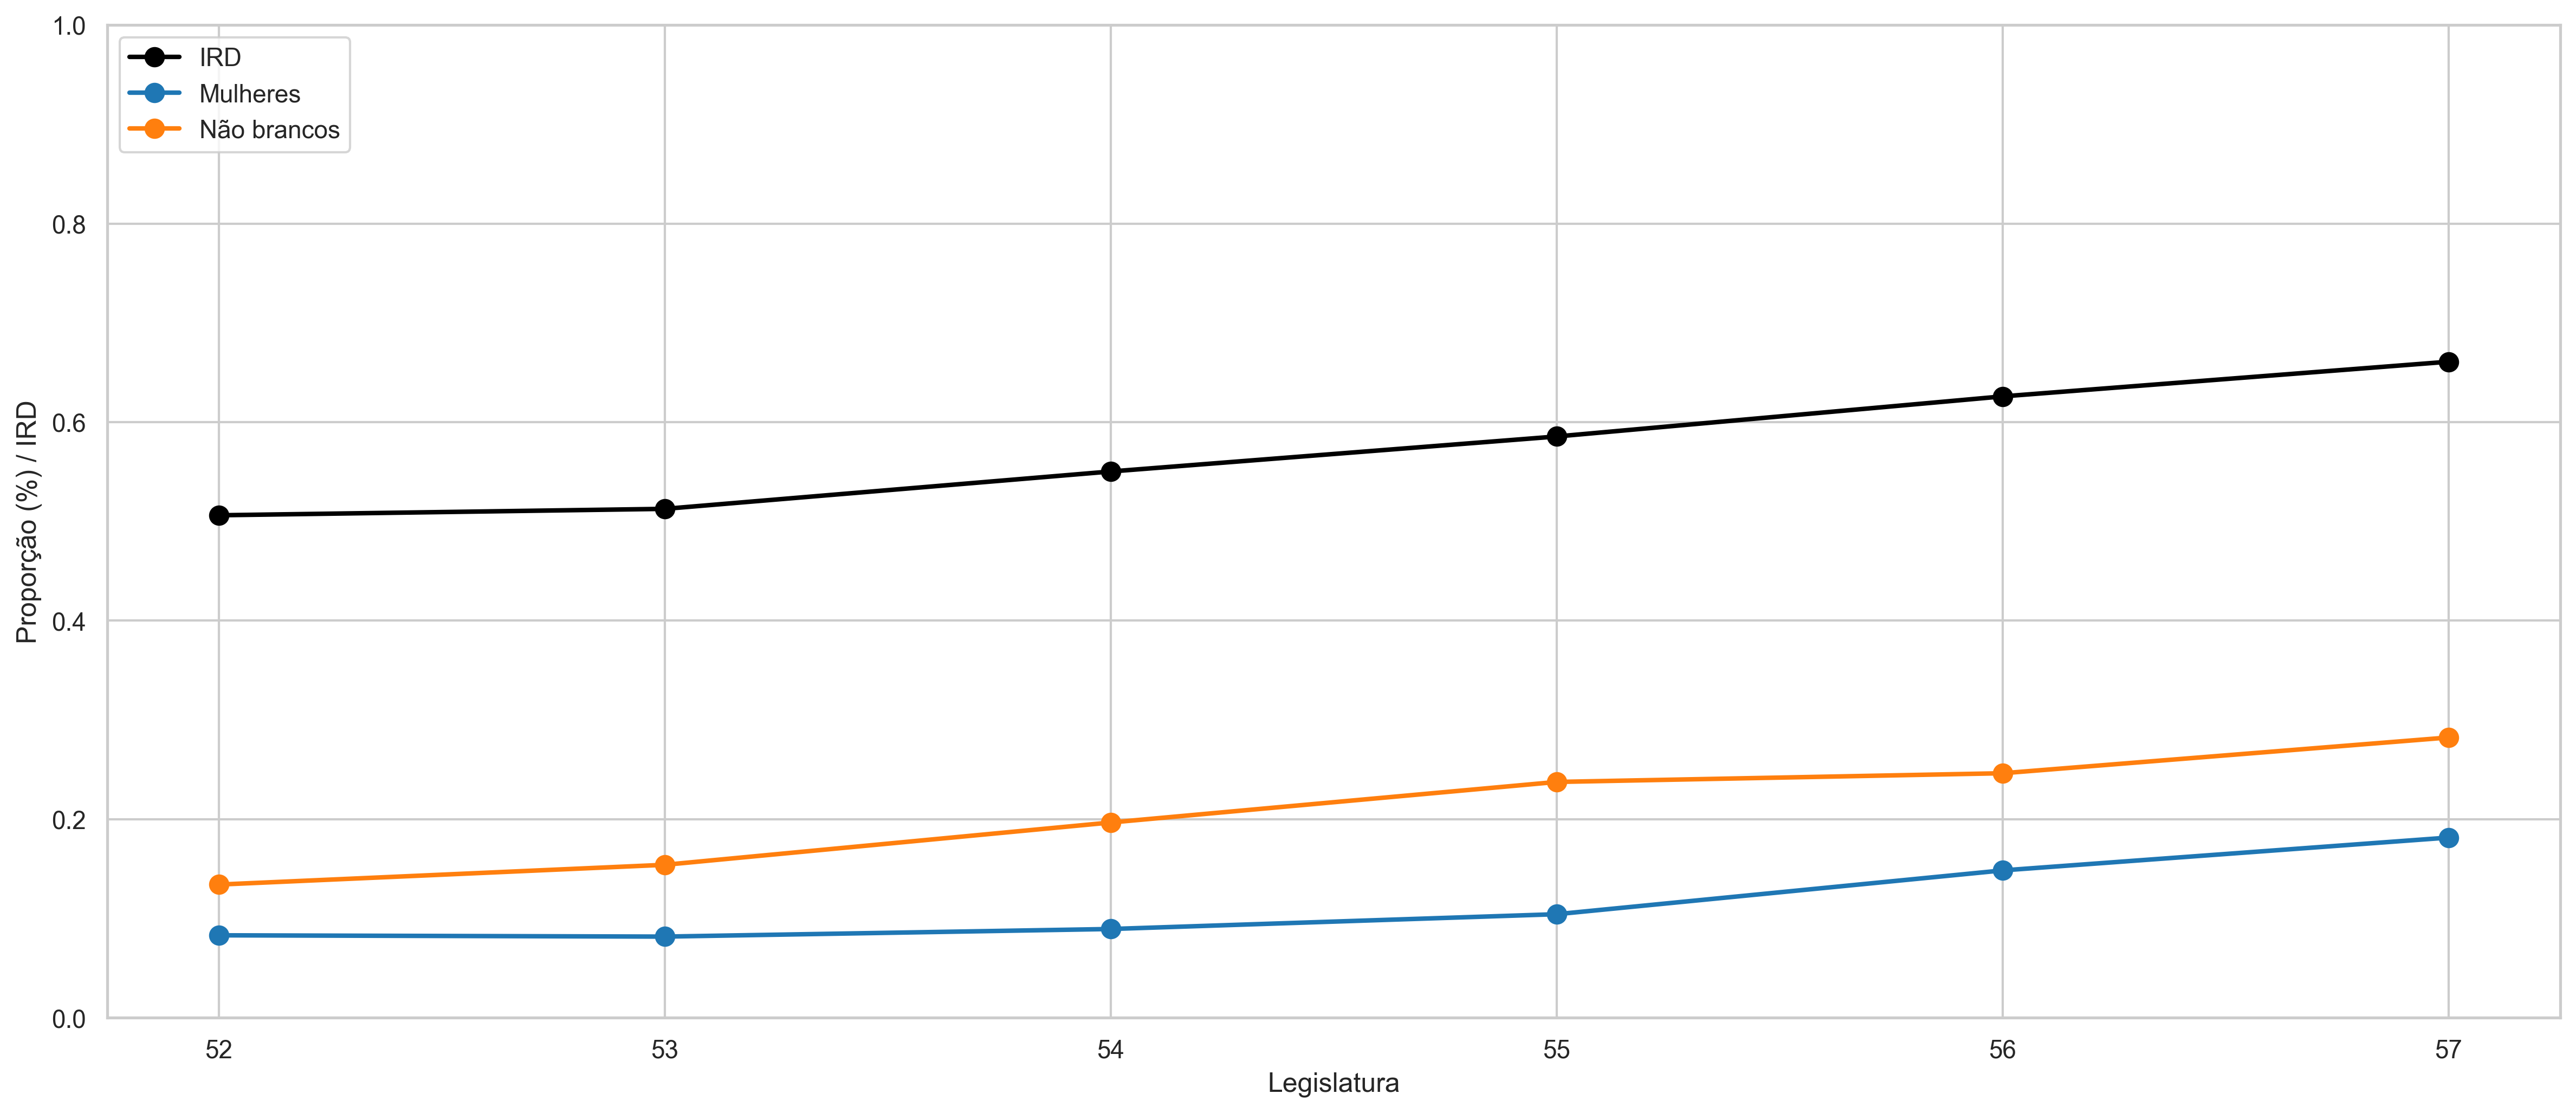
\includegraphics[width=0.8\textwidth]{figures/ird_vs_time.png}
    \caption{Evolução do Índice de Representação Descritiva (IRD) ao longo das legislaturas, demonstrando a correlação com o aumento da representação demográfica}
    \label{fig:ird_time}
\end{figure}

\subsubsection{Distribuição e Características do IRD}

A Figura \ref{fig:ird_distribution} apresenta a distribuição dos valores do IRD, permitindo analisar suas características estatísticas e a variabilidade entre diferentes períodos legislativos.

\begin{figure}
    \centering
    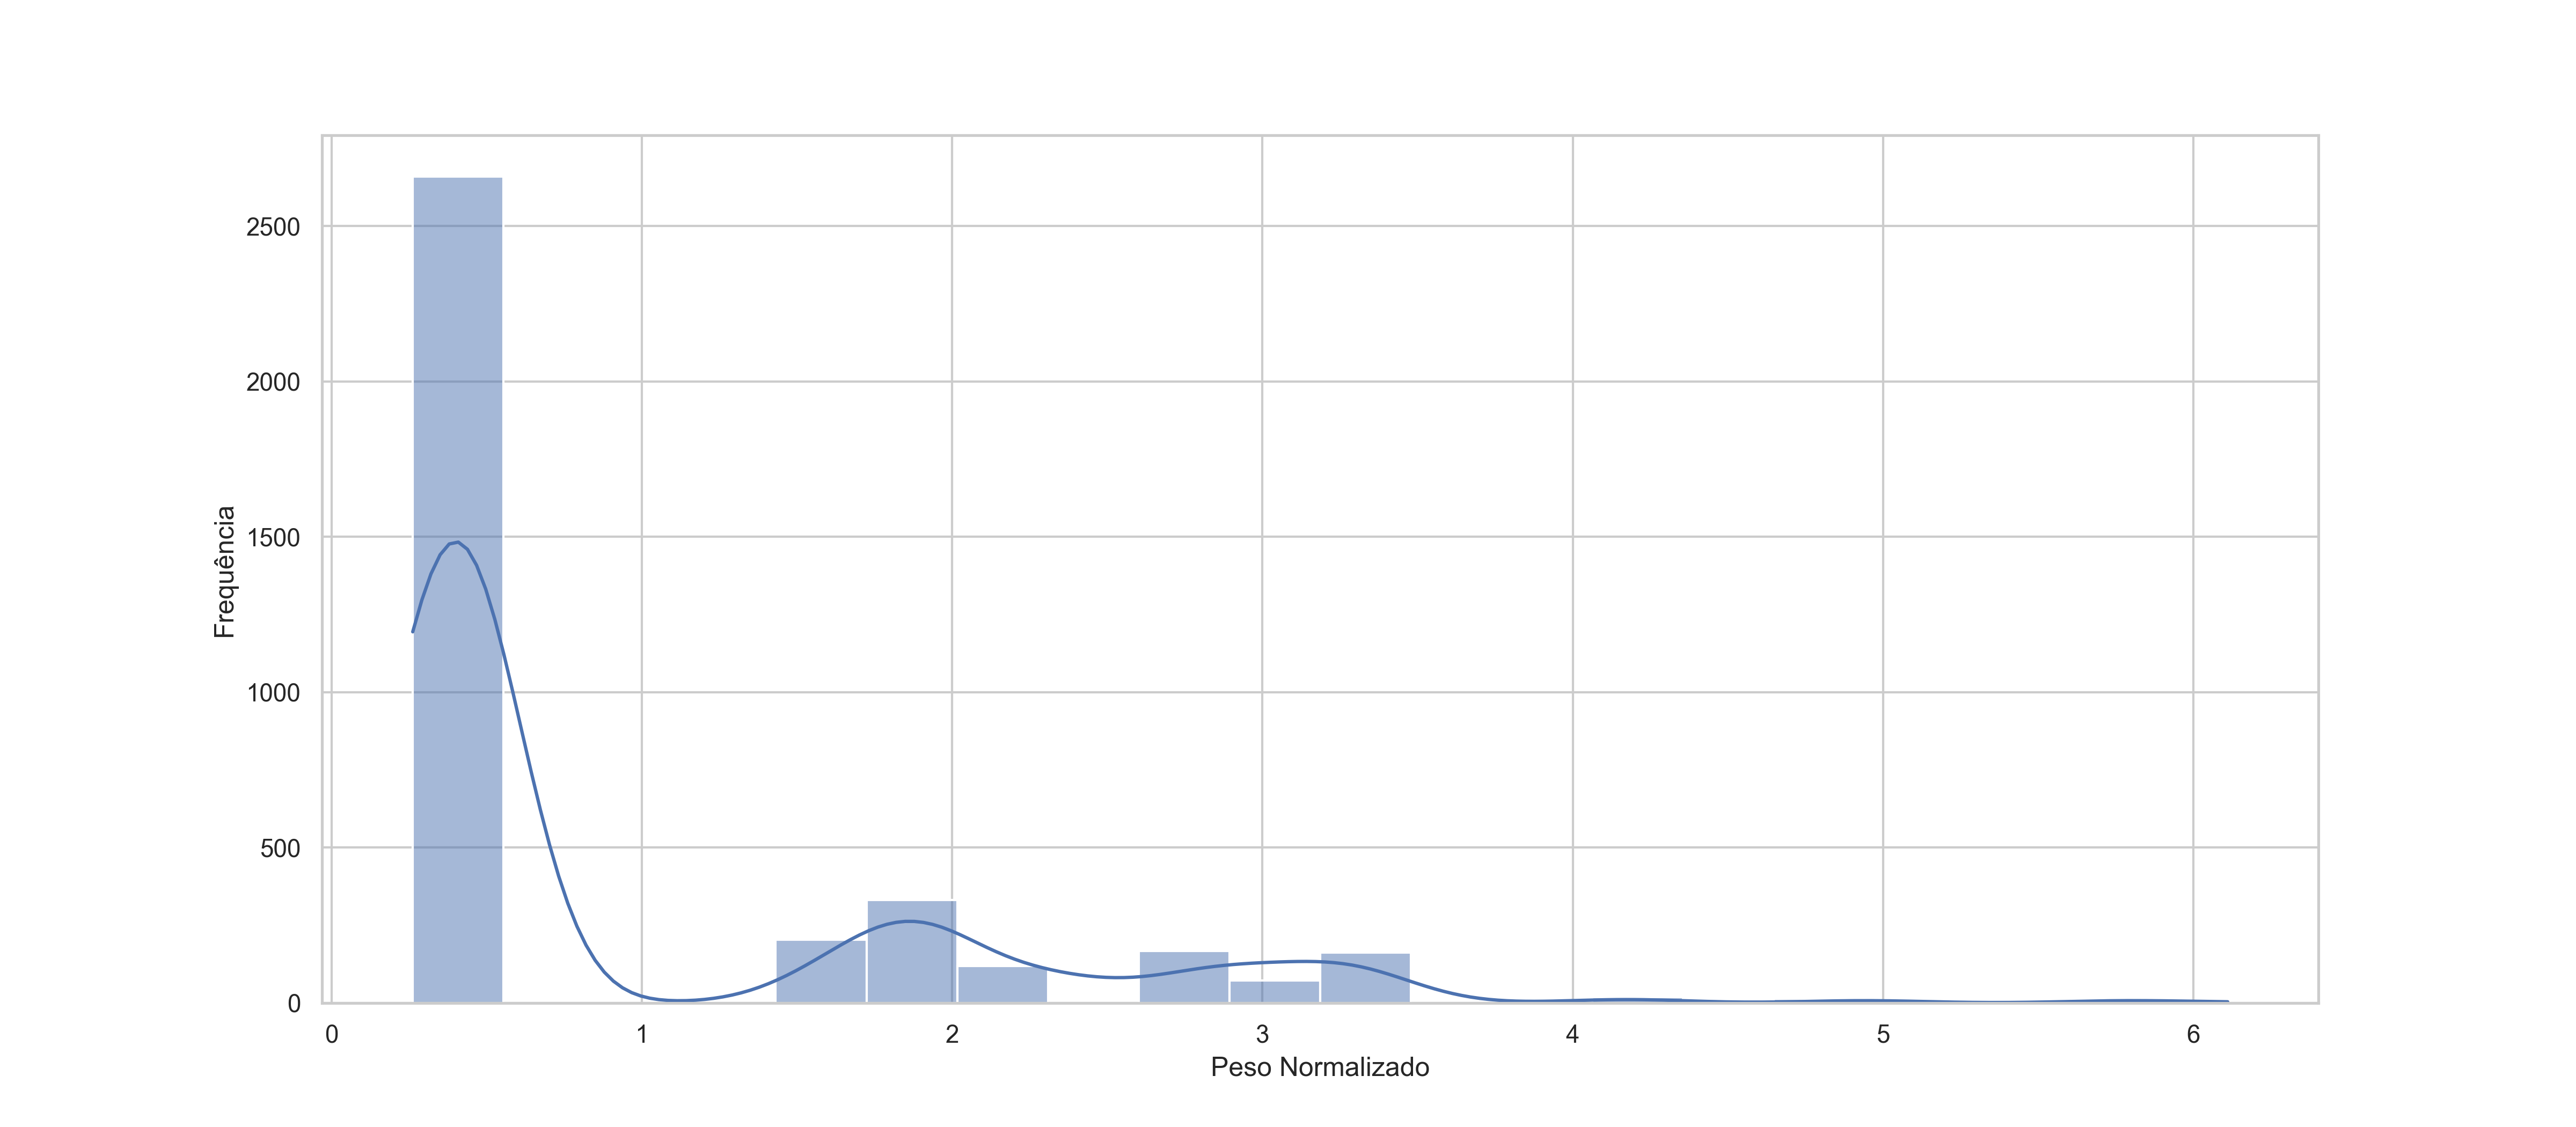
\includegraphics[width=0.8\textwidth]{figures/ird_distribution.png}
    \caption{Distribuição do Índice de Representação Descritiva (IRD) mostrando a variabilidade e padrões de representação demográfica ao longo do tempo}
    \label{fig:ird_distribution}
\end{figure}

A análise da distribuição do IRD revela padrões importantes sobre a representação descritiva no parlamento brasileiro:

\begin{itemize}
    \item \textbf{Forma da Distribuição}: A distribuição apresenta assimetria positiva, indicando que a maioria dos valores está concentrada em níveis mais baixos de representação descritiva
    \item \textbf{Variabilidade}: Existe considerável variabilidade nos valores do IRD, refletindo diferenças significativas na representação demográfica entre diferentes períodos e contextos políticos
    \item \textbf{Concentração}: Os valores tendem a se concentrar em faixas específicas, sugerindo padrões consistentes de representação ao longo do tempo
\end{itemize}

Os valores do IRD podem ser interpretados da seguinte forma:

\begin{itemize}
    \item \textbf{Valores Baixos (0.0 - 0.3)}: Indicam baixa representação descritiva, com significativa sub-representação de grupos demográficos
    \item \textbf{Valores Médios (0.3 - 0.7)}: Representam representação moderada, com algum equilíbrio entre grupos demográficos
    \item \textbf{Valores Altos (0.7 - 1.0)}: Indicam alta representação descritiva, com boa proporcionalidade demográfica
\end{itemize}

A distribuição do IRD revela importantes implicações para a democracia brasileira:

\begin{itemize}
    \item \textbf{Desafios Persistentes}: A concentração de valores em faixas mais baixas indica que a sub-representação demográfica persiste como um desafio estrutural
    \item \textbf{Progresso Gradual}: A presença de valores mais altos em alguns períodos sugere que mudanças positivas são possíveis
    \item \textbf{Necessidade de Políticas}: A variabilidade observada sugere que políticas públicas podem efetivamente influenciar a representação descritiva
\end{itemize}

Comparando a distribuição do IRD com outros indicadores de representação:
